\begin{enumerate}[label=\thesubsection.\arabic*, ref=\thesubsection.\theenumi]
    \item
    \label{question:C10-Q01}
    \label{question-short:C10-Q01} If the quadratic equation $px^2-2\sqrt5\,px+15=0$ has two equal roots, find $p$.
    
    \par
    \smallskip
    \solution

    For a repeated root, the two roots coincide precisely when the discriminant vanishes. Thus
    \begin{align*}
        \Delta & =(-2\sqrt5p)^2-4(p)(15)=20p^2-60p=20p(p-3)=0.
    \end{align*}

    The algebraic candidates are $p=0$ and $p=3$. The first candidate does not define a quadratic equation: its left side becomes $15$, which cannot be zero. Therefore the admissible parameter is
    \begin{align*}
        p & =3.
    \end{align*}

    As a root-finding check, set $F(x)=x(x-3)$. Newton--Raphson gives
    \begin{align*}
        x_{n+1} & =x_n-\frac{F(x_n)}{F'(x_n)}
    \end{align*}
    \hfill\eqref{formula:C10-Q01-F02}

    \par
    \begin{align*}
        & =x_n-\frac{x_n(x_n-3)}{2x_n-3}.
    \end{align*}

    At the desired simple root $x=3$, $F'(3)=3\ne0$ and the Newton map has the expected local quadratic convergence; the singular midpoint $x=3/2$ must be avoided.

    \begin{align*}
        p & =3
    \end{align*}

    \begin{figure}[H]
        \centering
        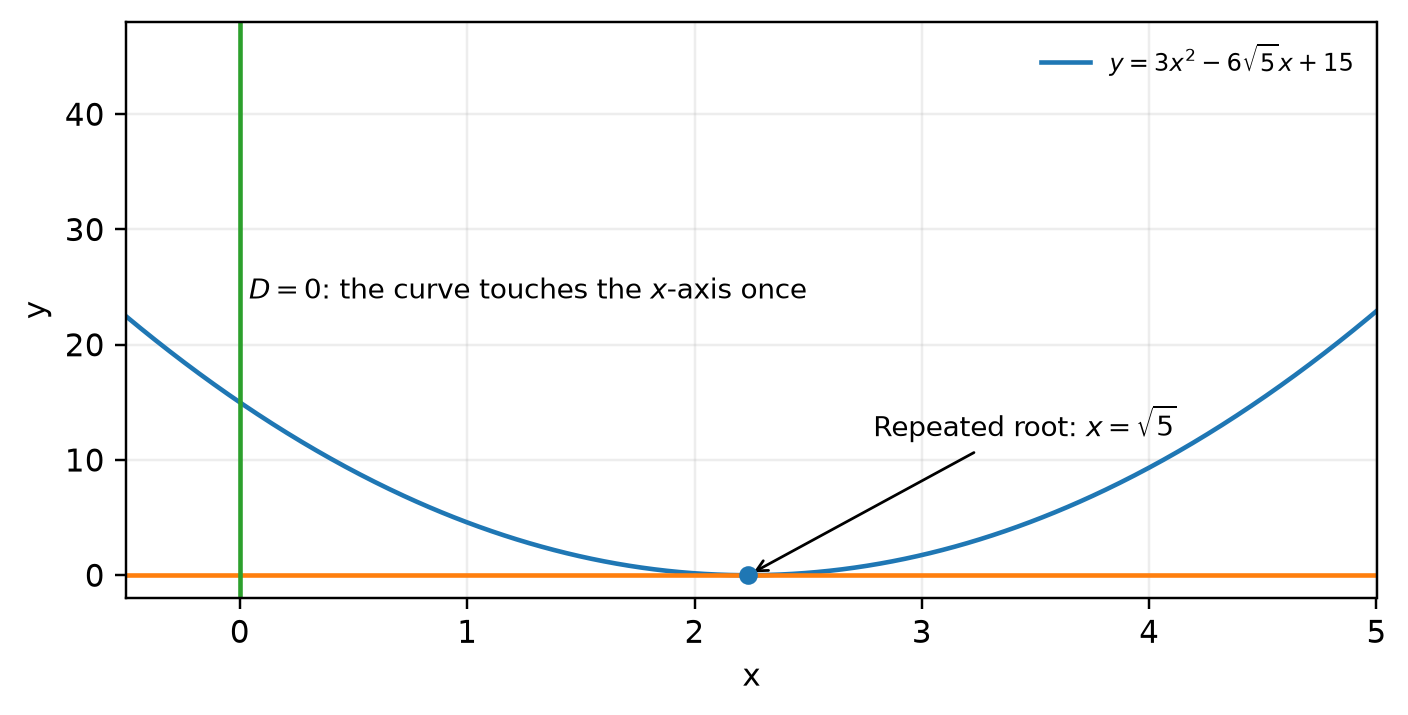
\includegraphics[width=0.92\linewidth]{10/figs/Q01.png}
    \end{figure}

    The following code verifies the solution.
\\
    \begin{lstlisting}[frame=single, basicstyle=\rmfamily, escapeinside={(*@}{@*)}]
(*@\makebox[\dimexpr\linewidth-2\fboxsep-2\fboxrule\relax][c]{10/codes/Q01.py}@*)
    \end{lstlisting}


    \item
    \label{question:C10-Q03}
    \label{question-short:C10-Q03} Two different dice are tossed together. Find the probability that the product of their top numbers is $6$.

    \par
    \smallskip
    \solution

    Let $X$ and $Y$ be the independent outcomes of the two fair dice. Their joint mass function is
    \begin{align*}
        P(X=i,Y=j) & =P(X=i)P(Y=j)
    \end{align*}
    \hfill\eqref{formula:C10-Q03-F01}

    \par
    \begin{align*}
        & =\frac1{36},\qquad 1\le i,j\le6.
    \end{align*}

    The product is a discrete push-forward random variable. Its probability is therefore obtained by summing the joint mass over the product preimage:
    \begin{align*}
        P(XY=z) & =\sum_{ij=z}P(X=i,Y=j).
    \end{align*}
    \hfill\eqref{formula:C10-Q03}

    \par
    For $z=6$, the admissible ordered pairs are
    \begin{align*}
        \{(i,j):ij & =6\}=\{(1,6),(2,3),(3,2),(6,1)\}.
    \end{align*}

    There are four equally likely pairs out of $6\times6=36$, so
    \begin{align*}
        P(XY=6) & =4\left(\frac1{36}\right)=\frac4{36}=\frac19.
    \end{align*}


    \begin{figure}[H]
        \centering
        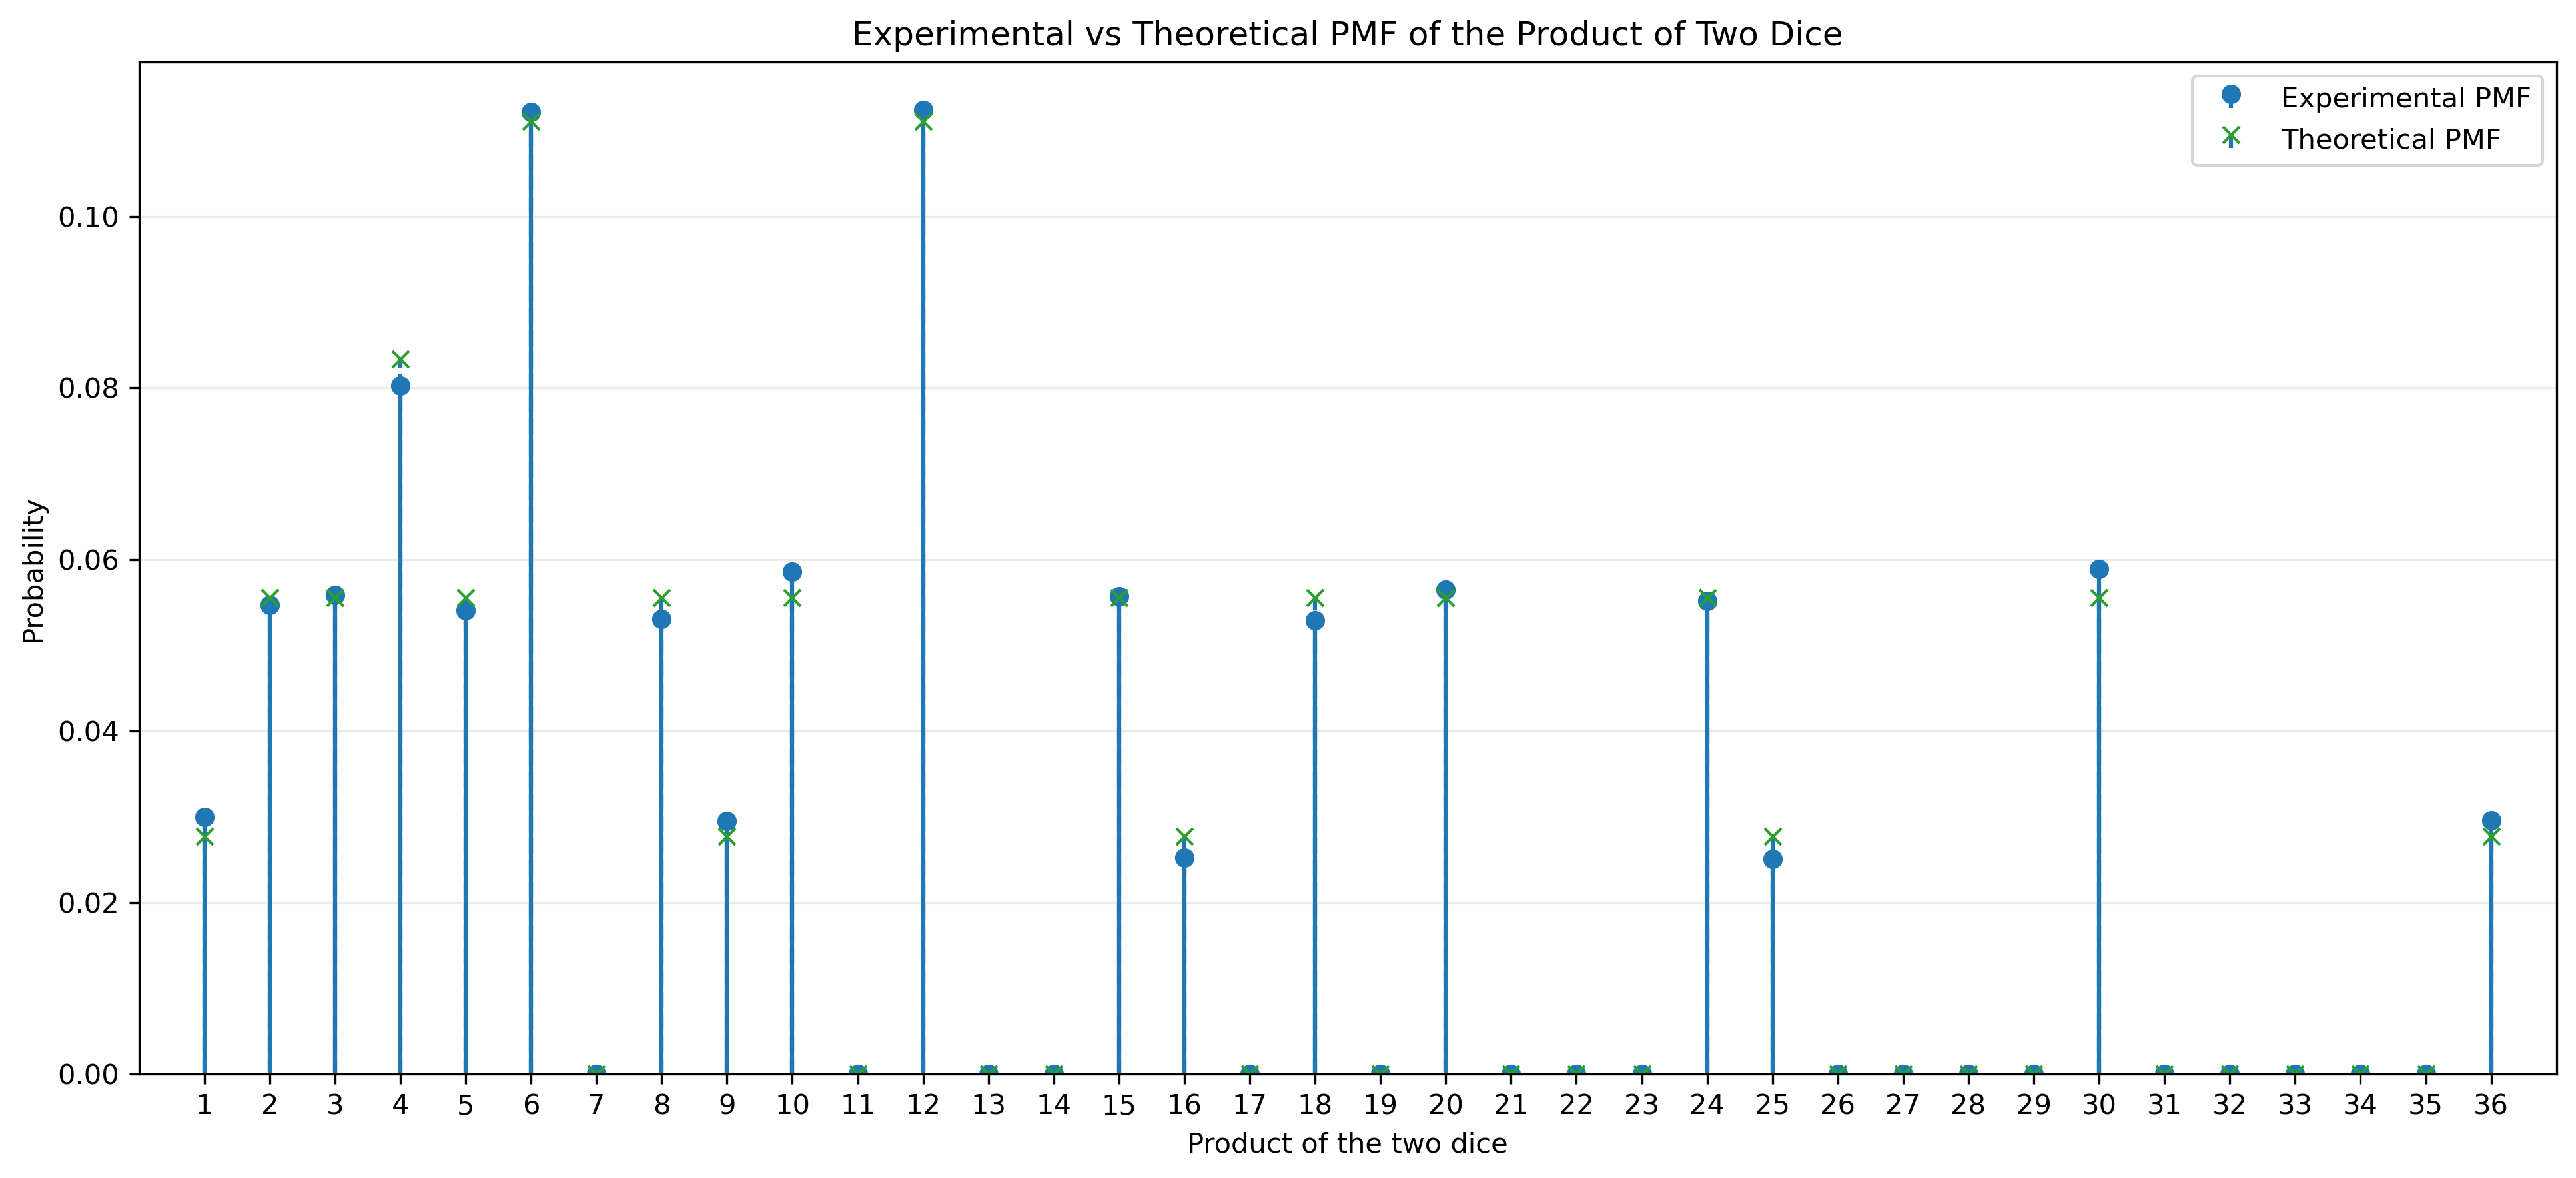
\includegraphics[width=0.98\linewidth]{10/figs/Q03.png}
    \end{figure}

    The following code generates random variables for the experimental plot.

     \begin{lstlisting}[frame=single, basicstyle=\rmfamily, escapeinside={(*@}{@*)}]
(*@\makebox[\dimexpr\linewidth-2\fboxsep-2\fboxrule\relax][c]{10/codes/Q03/dice\_simulation.c}@*)
    \end{lstlisting}

    The following code verifies the solution.

    \begin{lstlisting}[frame=single, basicstyle=\rmfamily, escapeinside={(*@}{@*)}]
(*@\makebox[\dimexpr\linewidth-2\fboxsep-2\fboxrule\relax][c]{codes/C10/Q03/Q03.py}@*)
    \end{lstlisting}



	\item \label{question:C10-Q08}\label{question-short:C10-Q08}
	In an arithmetic progression, $S_5+S_7=167$ and $S_{10}=235$. Find the AP.
	      \par\smallskip\solution
	      Let $a$ be the first term and $d$ be the common difference of the AP.
	      The sum of the first $n$ terms is
	      \begin{align*}
		      S_n & =\frac n2\bigl(2a+(n-1)d\bigr).
	      \end{align*}
	      \hfill\eqref{formula:C10-Q08-F01}\par

	      Substituting the given values,
	      \begin{align*}
		      S_5+S_7
		      & =(5a+10d)+(7a+21d) \\
		      & =12a+31d=167. \\
		      S_{10}
		      & =10a+45d=235.
	      \end{align*}

	      Writing $\vec{x}=\myvec{a\\d}$, the system of linear equations can be expressed as
	      \begin{align*}
		      A\vec{x} & =\vec{b}.
	      \end{align*}
	      \hfill\eqref{formula:C10-Q08}\par

	      where
	      \begin{align*}
		      A &= \myvec{12&31\\10&45} &
		      \vec{b} &= \myvec{167\\235}.
	      \end{align*}

	      Applying Gaussian elimination to the augmented matrix,
	      \begin{align*}
		      \left[\begin{array}{cc|c}
			      12 & 31 & 167 \\
			      10 & 45 & 235
		      \end{array}\right]
		      &\xrightarrow{\substack{R_1\rightarrow5R_1\\R_2\rightarrow6R_2}}
		      \left[\begin{array}{cc|c}
			      60 & 155 & 835 \\
			      60 & 270 & 1410
		      \end{array}\right] \\[6pt]
		      &\xrightarrow{R_2\rightarrow R_2-R_1}
		      \left[\begin{array}{cc|c}
			      60 & 155 & 835 \\
			      0 & 115 & 575
		      \end{array}\right].
	      \end{align*}

	      \begin{align*}
		      A'\vec{x} & =\vec{b'}
	      \end{align*}
	      
	       \begin{align*}
		      A' &= \myvec{60&155\\0&115} &
		       \vec{b'} &= \myvec{835\\575}.
	      \end{align*}

	      From the second row,
	      \begin{align*}
		      115d &=575,\\
		      d &=5.
	      \end{align*}

	      Substituting $d=5$ into the first equation,
	      \begin{align*}
		      12a+31(5) &=167,\\
		      12a &=12,\\
		      a &=1.
	      \end{align*}

	      Therefore, the first term is $1$ and the common difference is $5$.
	      The required AP is
	      \begin{align*}
		      1,6,11,16,21,26,31,\ldots
	      \end{align*}

	      The general term is
		\begin{align*}
			x(n) &= (a+(n-1)d)u(n-1).
		\end{align*}
		\hfill\eqref{formula:C10-Q08-F03}\par

		\begin{align*}
			x(n) &= (1+5(n-1))u(n-1)\\
			&= (5n-4)u(n-1).
		\end{align*}
		
		\[
u(n-1) =
\begin{cases}
1, & n \geq 1,\\
0, & \text{otherwise}.
\end{cases}
\]

	      Verifying the given conditions,
	      \begin{align*}
		      S_5 &=5(1)+10(5)=55,\\
		      S_7 &=7(1)+21(5)=112,\\
		      S_5+S_7 &=55+112=167,\\
		      S_{10} &=10(1)+45(5)=235.
	      \end{align*}

	      Both conditions are satisfied. The following code verifies the solution.
	      \begin{lstlisting}[frame=single, basicstyle=\rmfamily, escapeinside={(*@}{@*)}]
(*@\makebox[\dimexpr\linewidth-2\fboxsep-2\fboxrule\relax][c]{10/codes/Q08.py}@*)
\end{lstlisting}

    \item
    \label{question:C10-Q10}
    \label{question-short:C10-Q10} If $A(x,y)$, $B(-5,7)$ and $C(-4,5)$ are collinear, find the relation between $x$ and $y$.

    \par
    \smallskip
    \solution

     Since the points $A$, $B$ and $C$ are collinear, the displacement vectors
	      $\overrightarrow{\vec{AB}}$ and $\overrightarrow{\vec{AC}}$ are linearly dependent.
	      Therefore, the matrix formed by these vectors has rank $1$.

	      \begin{align*}
		      M &= \myvec{-5-x & 7-y\\-4-x & 5-y}.
	      \end{align*}

	      Applying elementary row operations to obtain row echelon form,

	      \begin{align*}
		      M &\xrightarrow{R_2\rightarrow R_2-R_1}
		      \myvec{-5-x & 7-y\\1 & -2}\\[6pt]
		        &\xrightarrow{R_1\leftrightarrow R_2}
		      \myvec{1 & -2\\-5-x & 7-y}\\[6pt]
		        &\xrightarrow{R_2\rightarrow R_2+(x+5)R_1}
		      \myvec{1 & -2\\0 & -2x-y-3}.
	      \end{align*}

	      Since the rank of the matrix is $1$, the second row in its row echelon form must be a zero row.

	      Therefore,
	      \begin{align*}
		      -2x-y-3 &= 0.
	      \end{align*}

	      Hence, the required relation between $x$ and $y$ is
	      \begin{align*}
		      2x+y+3 &= 0.
	      \end{align*}
	       \begin{figure}[H]
        \centering
        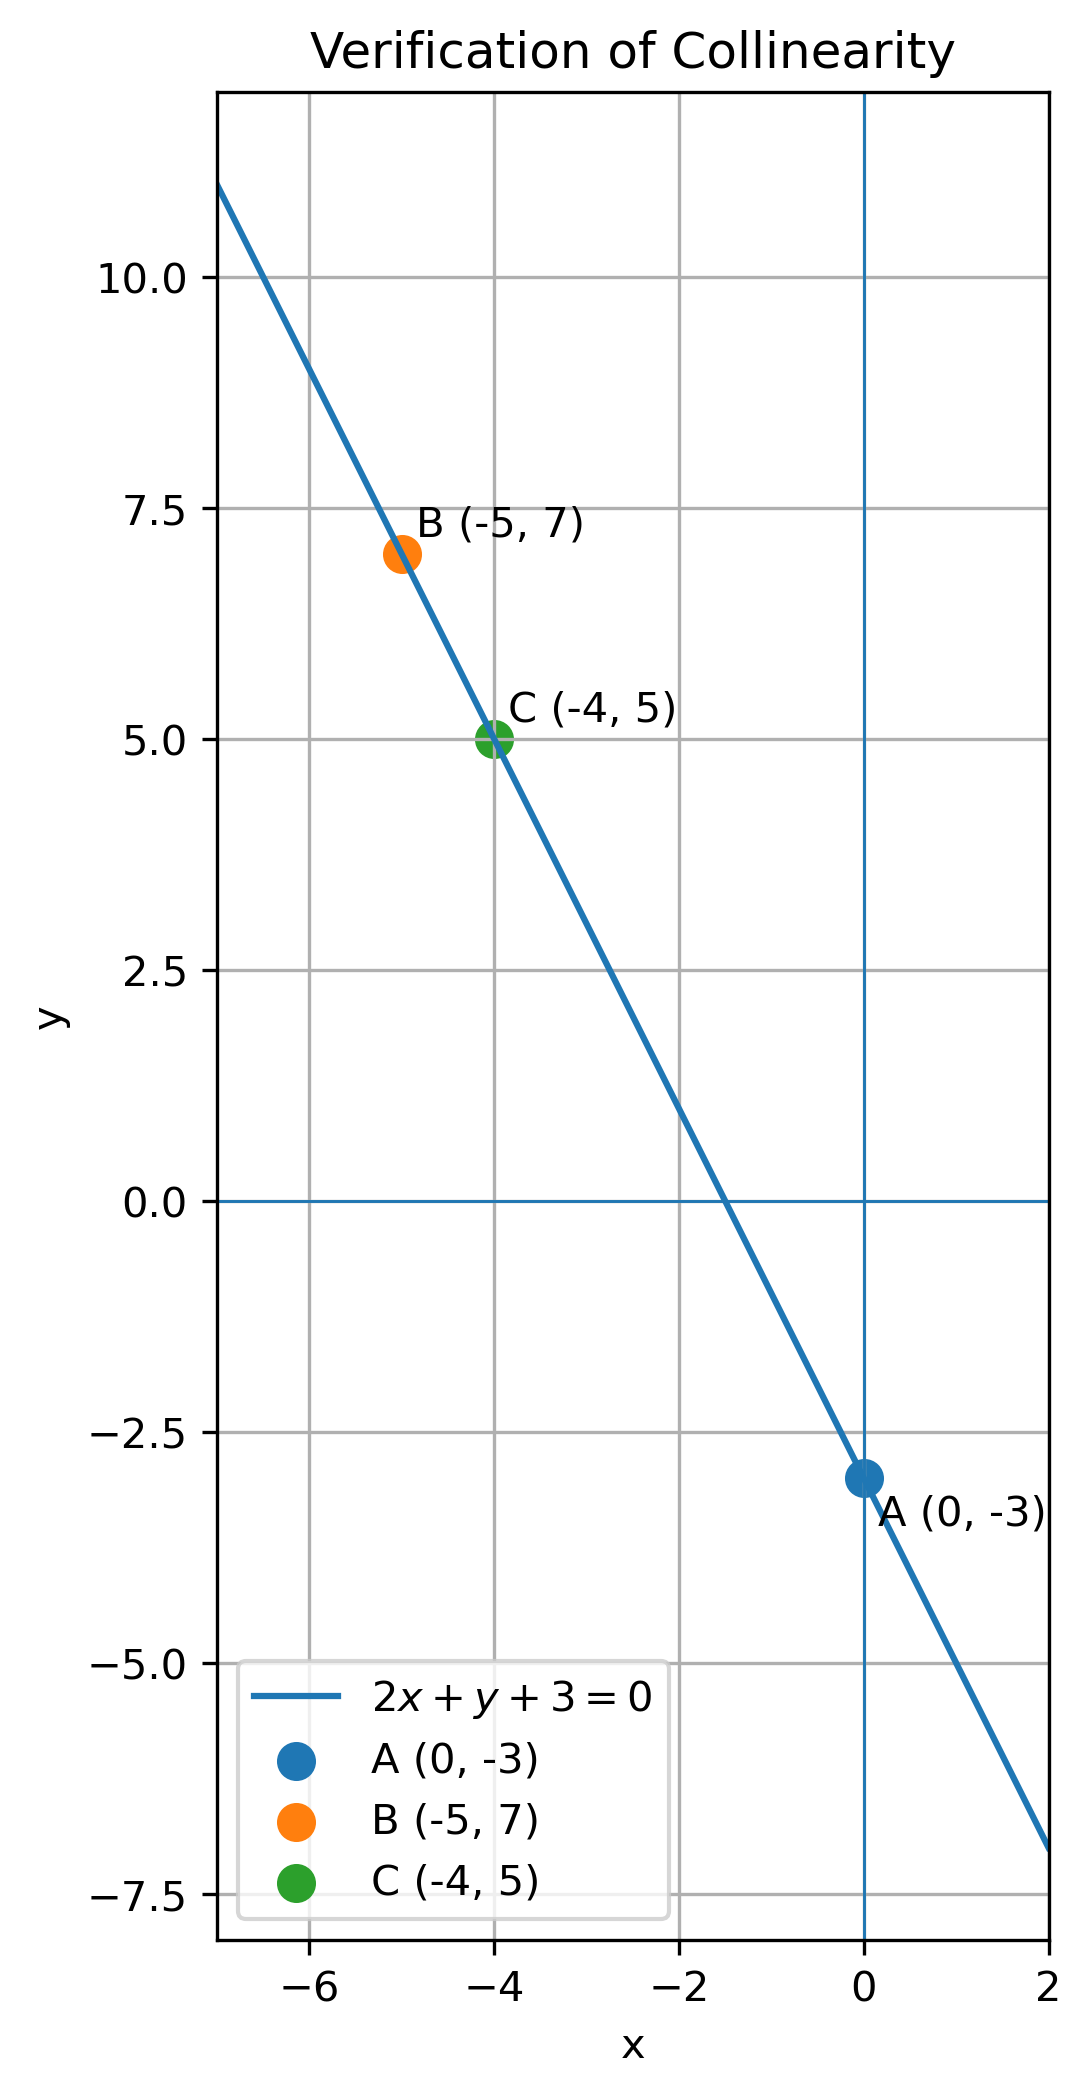
\includegraphics[width=0.3\linewidth]{10/figs/Q10.png}
    \end{figure}

     \begin{lstlisting}[frame=single, basicstyle=\rmfamily, escapeinside={(*@}{@*)}]
(*@\makebox[\dimexpr\linewidth-2\fboxsep-2\fboxrule\relax][c]{10/codes/Q10.py}@*)
\end{lstlisting}


    \item
    \label{question:C10-Q11}
    \label{question-short:C10-Q11} The 14th term of an AP is twice its 8th term. If the 6th term is $-8$, find the sum of its first 20 terms.

    \par
    \smallskip
    \solution

    Model the AP as the discrete-time sequence $x[n]=(a+(n-1)d)u(n-1)$, $n\ge1$. Its unilateral transform separates the constant and ramp components:
    \begin{align*}
	    X(z) & =\sum_{n=1}^{\infty}x(n)z^{-n}=\frac{az^{-1}}{1-z^{-1}}+\frac{dz^{-2}}{(1-z^{-1})^2}.
    \end{align*}
    \hfill\eqref{formula:C10-Q11}

    \[
u(n-1) =
\begin{cases}
1, & n \geq 1,\\
0, & \text{otherwise}.
\end{cases}
\]
    \par
    The term conditions give two linear equations:
    \begin{align*}
        a+13d & =2(a+7d),\qquad a+5d=-8.
    \end{align*}

    The first equation reduces to $a+d=0$, so $a=-d$. Substitution into the second equation gives
    \begin{align*}
        a+13d & =2(a+7d). \\
        a+5d  & =-8.
    \end{align*}

    The twentieth partial sum is consequently
    \begin{align*}
        S_{20} & =\frac{20}{2}\bigl(2a+19d\bigr)=10(4-38)=-340.
    \end{align*}

    The sequence generated by $(a,d)=(2,-2)$ has $t_6=-8$ and $t_{14}=-24=2t_8$, confirming both data constraints.

    The following code verifies the solution.

    \begin{lstlisting}[frame=single, basicstyle=\rmfamily, escapeinside={(*@}{@*)}]
(*@\makebox[\dimexpr\linewidth-2\fboxsep-2\fboxrule\relax][c]{10/codes/Q11.py}@*)
    \end{lstlisting}


    \item
    \label{question:C10-Q15}
    \label{question-short:C10-Q15} A jar contains only red, blue and orange balls. The probabilities of drawing a red and a blue ball are $\frac14$ and $\frac13$, respectively. If there are 10 orange balls, find the total number of balls.

    \par
    \smallskip
    \solution


	Let $X$ be a discrete random variable representing the colour of the ball drawn from the jar, where

	\begin{align*}
	X &=
	\begin{cases}
	1, & \text{Red},\\
	2, & \text{Blue},\\
	3, & \text{Orange}.
	\end{cases}
	\end{align*}

	The given probabilities are
	\begin{align*}
	P(X=1) &= \frac14,\\
	P(X=2) &= \frac13.
	\end{align*}

	Since the jar contains only red, blue and orange balls, these outcomes are mutually exclusive and exhaustive. Therefore, the sum of their probabilities must be unity.

	\begin{align*}
	P(X=1)+P(X=2)+P(X=3) &= 1, \hfill\eqref{formula:C10-Q15}	\\
	\frac14+\frac13+P(X=3) &= 1,\\
	P(X=3) &= 1-\frac14-\frac13\\
	&= \frac5{12}.
	\end{align*}

	Let $N$ be the total number of balls in the jar. Since there are 10 orange balls, the probability of drawing an orange ball is

	\begin{align*}
	P(X=3) &= \frac{\text{Number of orange balls}}{\text{Total number of balls}}\\
	\frac5{12} &= \frac{10}{N},\\
	5N &= 120,\\
	N &= 24.
	\end{align*}

	Thus, the total number of balls in the jar is
	\begin{align*}
	N=24.
	\end{align*}

	The probability mass function of $X$ is

	\begin{align*}
	p_X(x) &=
	\begin{cases}
	\frac14, & x=1,\\[3pt]
	\frac13, & x=2,\\[3pt]
	\frac5{12}, & x=3,\\[3pt]
	0, & \text{otherwise}.
	\end{cases}
	\end{align*}
	
	The PMF satisfies the normalization condition
	\begin{align*}
	\sum_x p_X(x) &= \frac14+\frac13+\frac5{12}\\
	&= 1.
	\end{align*}
    
    \begin{figure}[H]
        \centering
        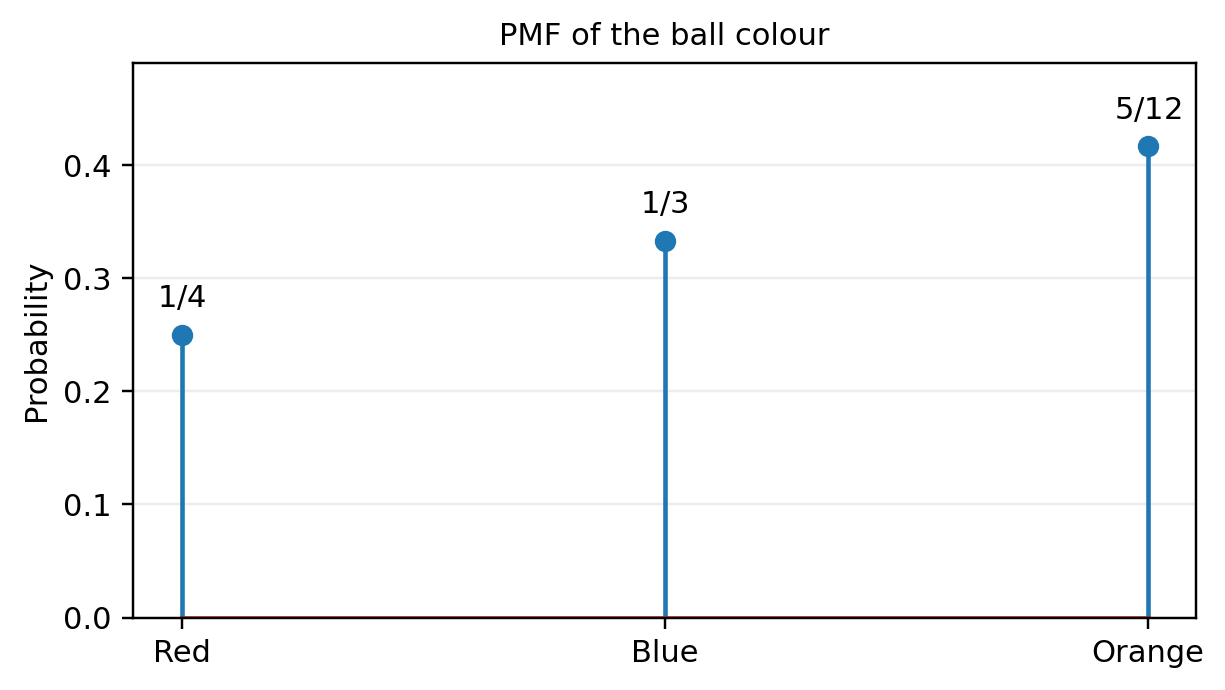
\includegraphics[width=0.9\linewidth]{10/figs/Q15.png}
    \end{figure}

    The following code verifies the solution.

    \begin{lstlisting}[frame=single, basicstyle=\rmfamily, escapeinside={(*@}{@*)}]
(*@\makebox[\dimexpr\linewidth-2\fboxsep-2\fboxrule\relax][c]{10/codes/Q15.py}@*)
    \end{lstlisting}


    \item
    \label{question:C10-Q22}
    \label{question-short:C10-Q22} Find the 60th term of the AP $8,10,12,\ldots$ and the sum of its last 10 terms.

    \par
    \smallskip
    \solution

    Index the finite AP from zero so that $x(n)=(8+2n)u(n)$ for $0\le n\le59$. The finite-support signal, rather than an infinite extension, is represented by
    \begin{align*}
        X(z) & =8\sum_{n=0}^{59}z^{-n}+2\sum_{n=0}^{59}nz^{-n}.
    \end{align*}
    \hfill\eqref{formula:C10-Q22}\par

    \[
u(n) =
\begin{cases}
1, & n \geq 0,\\
0, & \text{otherwise}.
\end{cases}
\]

    The requested term is the sample at the final index:
    \begin{align*}
	    x(59) & =8+2(59)=126.
    \end{align*}

    The last ten terms are indexed by $n=50,\ldots,59$, with
    \begin{align*}
	    x(50) & =8+100=108. \\
	    x(59) & =126.
    \end{align*}

    Using the arithmetic-series sum,
    \begin{align*}
	    \sum_{n=50}^{59}x(n) & =\frac{10}{2}(108+126)=5(234)=1170.
    \end{align*}

    The finite index range confirms that no samples beyond the 60-term support have entered the calculation.

    The following code verifies the solution.

    \begin{lstlisting}[frame=single, basicstyle=\rmfamily, escapeinside={(*@}{@*)}]
(*@\makebox[\dimexpr\linewidth-2\fboxsep-2\fboxrule\relax][c]{10/codes/Q22.py}@*)
    \end{lstlisting}


    \item
    \label{question:C10-Q28}
    \label{question-short:C10-Q28} A card is drawn from a well-shuffled 52-card deck. Find the probability that it is (i) a spade or an ace, (ii) a black king, (iii) neither a jack nor a king, (iv) either a king or a queen.

    \par
    \smallskip
    \solution

    Use indicator variables to preserve the overlap correction in unions. For a spade $S$ and an ace $A$, $|S|=13$, $|A|=4$, and $|S\cap A|=1$. Thus
    \begin{align*}
        \mathbf 1_{S\cup A} & =\mathbf 1_S+\mathbf 1_A-\mathbf 1_{S\cap A}.
    \end{align*}
    \hfill\eqref{formula:C10-Q28}

    \par
    \begin{align*}
        P(S\cup A) & =\frac{|S|+|A|-|S\cap A|}{52}.
    \end{align*}

    The four requested probabilities follow from the corresponding event counts:
    \begin{align*}
        P(S\cup A)                      & =\frac{13+4-1}{52}=\frac4{13}.                 \\
        P(\text{black king})            & =\frac2{52}=\frac1{26}.                        \\
        P(\text{neither jack nor king}) & =1-\frac{4+4}{52}=\frac{44}{52}=\frac{11}{13},
    \end{align*}

    and, since kings and queens are disjoint,
    \begin{align*}
        P(K\cup Q) & =\frac{4+4}{52}=\frac2{13}.
    \end{align*}

    Hence the answers are
    \begin{align*}
        \frac4{13},\quad \frac1{26},\quad \frac{11}{13},\quad \frac2{13}.
    \end{align*}


\end{enumerate}
